\section{Tabelas e Figuras}

\begin{frame}{Tabelas}
  Você pode usar tabelas, tal como a Tabela \ref{tab:parametros}.

  \vspace{2mm}

  \begin{table}[h]
    \centering
    \begin{tabular}{l c c}
      \hline
      Parâmetro   & Valor & Unidade                 \\
      \hline
      Pressão     & 5.0   & bar                     \\
      Temperatura & 298   & K                       \\
      Vazão       & 12.5  & \(\text{m}^3/\text{h}\) \\
      \hline
    \end{tabular}
    \caption{Parâmetros operacionais básicos}
    \label{tab:parametros}
  \end{table}
\end{frame}

\begin{frame}{Figuras}
  Você pode incluir figuras facilmente, como mostrado na Figura \ref{fig:pendulo}.

  \vspace{2mm}

  \begin{figure}[h]
    \centering
    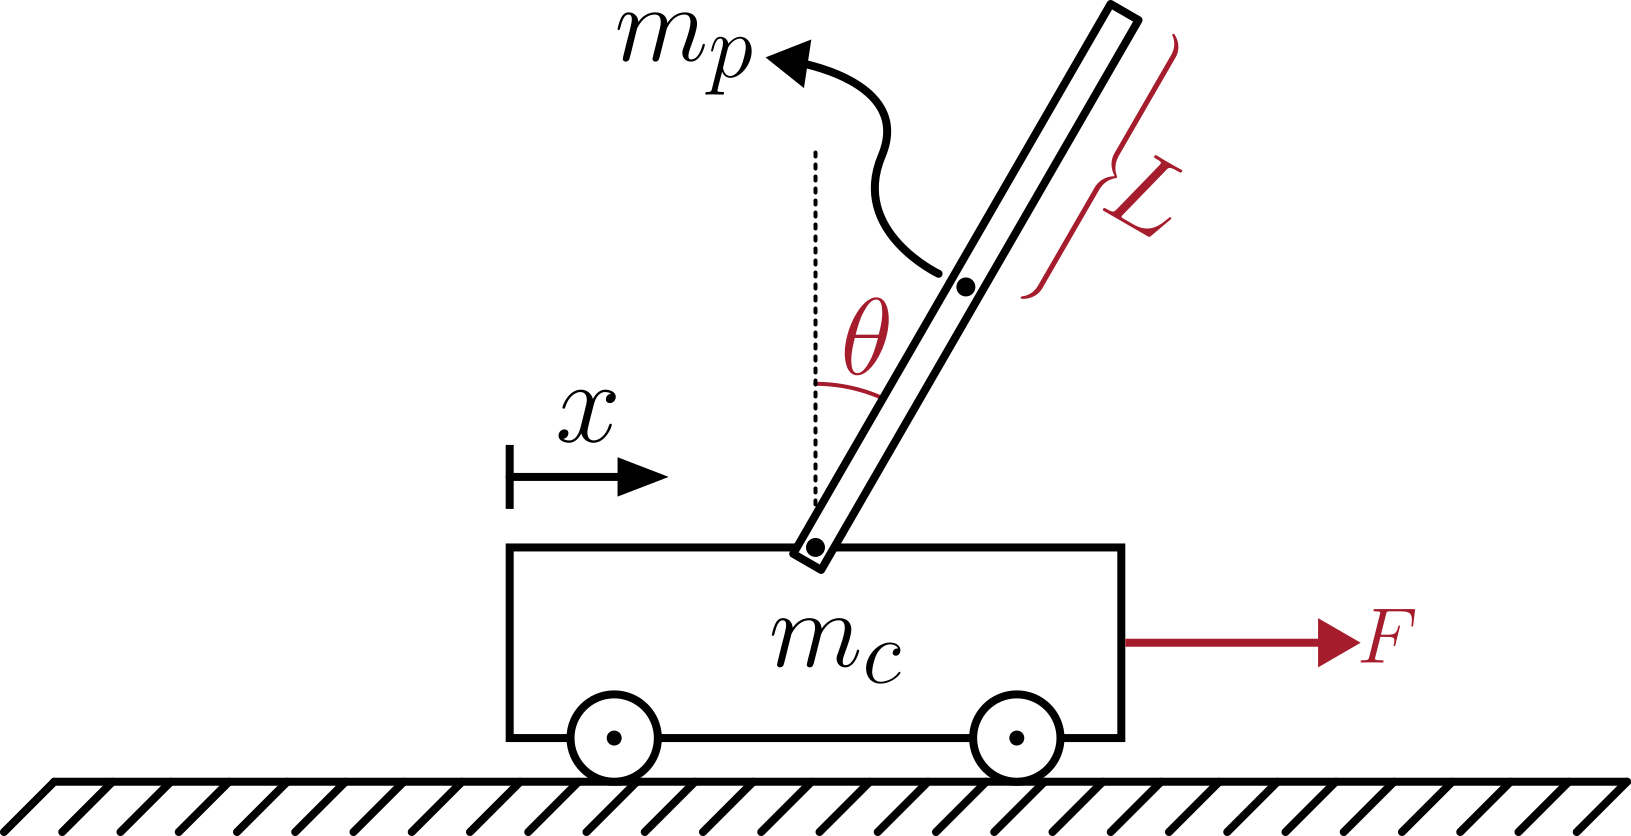
\includegraphics[width=0.6\textwidth]{figures/example.png}
    \caption{Representação do sistema físico de um pêndulo invertido.}
    \label{fig:pendulo}
  \end{figure}
\end{frame}
